% Abstract file structure example : 
% \abstitle{title here}
% \absauthors{names and superscripts for affiliations here}
% \absaddress{affiliations, starting each one with its superscripts, separate affiliations with a \break}
% \abstext{
% \index{author abbreviated name, to be placed in authors' index}
% \index{create an index entry for each author}
%  The abstract text
% }

%% Abstract title
%\abstitle{Studio sui chirotteri troglofili della Grotta di Calafarina (Pachino, SR, Sicilia sud-orientale)}

%% Author names
%\absauthors{M. \textsc{Mucedda}$^1$,  G. \textsc{Fichera}$^2$, E. \textsc{Pidinchedda}$^1$}

%\absaddress{$^1$Centro Pipistrelli Sardegna, Via G. Leopardi 1 – 07100 Sassari, Italy - batsar@tiscali.it\break
%$^2$Universität Trier Universitätsring,15 - D-54286  Trier, Germany}

%% Abstract text
%\abstext{
%%% Author names for index. State each author separately using \index{Doe J.}
%\index{Mucedda M.}
%\index{Fichera G.}
%\index{Pidinchedda E.}
%%% The actual abstract text goes here
%} %% remember to close the abstract text block brace!!
\label{ext:P001}

\loadabstr[E005]{DE PASQUALE P.P. -- La chirotterofauna dei boschi vetusti nel Parco Nazionale del Pollino}{abstracts/extended_abstracts/P005_depasquale_extended_title.tex}

\begin{multicols}{2}

\section*{Introduzione}
I boschi vetusti sono biocenosi in cui il disturbo antropico è assente o trascurabile, caratterizzate da una dinamica naturale che determina la presenza, al loro interno, di tutte le fasi di rigenerazione, compresa quella senescente con alberi di grandi dimensioni e abbondante necromassa (Blasi et al., 2010). Questi ambienti sono importanti per  le specie nemorali che beneficiano di bassi livelli di disturbo e della presenza di microhabitat (Nordén e Appelqvist, 2001), ma anche per numerose specie influenzate dalla presenza di necromassa legnosa (Christensen e Emborg, 1996), tra cui uccelli e chirotteri (Harmon et al., 1986).   

Almeno la metà delle specie di chirotteri presenti in Italia utilizza prevalentemente le foreste mature per il foraggiamento e per l’attività di \textit{roosting}. Il territorio del Parco Nazionale del Pollino è caratterizzato dalla presenza di almeno cinque formazioni forestali vetuste, che svolgono un ruolo ecologico fondamentale per numerose specie di chirotteri. Perciò è importante valutare le interazioni ecologiche tra questi mammiferi e gli habitat forestali. A tal proposito, il presente studio si pone l’obiettivo di fare un’analisi preliminare della comunità di chirotteri presente in queste biocenosi complesse, che sono potenzialmente in grado di regolarne il funzionamento.   

\section*{Materiali e metodi}
Le indagini di campo sono state condotte tra luglio ed agosto del 2015, in due boschi vetusti individuati nel versante lucano del massiccio del Pollino. I boschi sono stati censiti e caratterizzati durante il programma di ricerca finanziato dal MATTM e coordinato dall’Ente Parco Nazionale del Pollino, relativo alla costituzione della rete dei boschi vetusti nei Parchi in Italia meridionale.

Le formazioni forestali selezionate sono: il bosco misto di abete bianco (\emph{Abies alba}) e faggio (\emph{Fagus sylvatica}), il bosco misto di faggio e cerro (\emph{Quercus cerris}). Gli abieti-faggeti hanno una distribuzione piuttosto frammentaria in Italia meridionale e sono più frequenti solo nel territorio del Pollino e in Calabria (Ciancio et al., 1985). In particolare, la formazione oggetto di studio è localizzata prevalentemente nel territorio di Terranova del Pollino (PZ) ed è distribuita in una fascia altitudinale compresa tra 1350 e 1550 m s.l.m.; è costituita da 3 nuclei a bosco vetusto, compresi parzialmente nel bosco di Cugno dell’Acero e nel SIC IT9210075 ``Lago Duglia, Casino Toscano''. La cerreta-faggeta è presente nel territorio di San Severino lucano (PZ) e il nucleo a bosco vetusto è collocato nella fascia altitudinale compresa tra 700 e 900 m s.l.m.. La formazione forestale è denominata ``Bosco Magnano'' ed è compresa interamente nel SIC IT9210040 omonimo.

Il protocollo di ricerca ha previsto indagini mediante rilievi ultrasonori e catture temporanee in entrambe le tipologie forestali. I rilievi ultrasonori sono stati effettuati mediante un \textit{bat detector} in espansione temporale (10$\times$), modello Pettersson D240X. I campioni sono stati registrati mediante un registratore digitale Edirol R-09, con frequenza di campionamento a 44.1~kHz e risoluzione a 16~bit. L’attività dei chirotteri è stata quantificata rilevando il numero di passaggi di chirotteri per tipologia forestale attraverso il conteggio delle sequenze dei segnali di ecolocalizzazione (Fenton, 1970).

L’ordine di campionamento è stato effettuato in modo \textit{random} e in 15 punti d’ascolto per ogni tipologia di bosco; i punti sono stati selezionati anche nelle aree forestali a medesima consociazione limitrofe ai nuclei a bosco vetusto (Fig.~1) e il tempo di campionamento è stato di 15 minuti per punto, a partire da 30 minuti dopo il tramonto. L’attività dei chirotteri può essere influenzata dall’ora della notte e da fattori ambientali, come vento, pioggia, umidità, temperatura (Avery, 1985; Rydell, 1993; Vaughan et al., 1997; O’Donnell, 2000), per cui i rilievi ultrasonori sono stati effettuati nelle prime 4 ore della notte, fase in cui l’attività è più elevata e, solo durante le notti con temperature > a 10 °C, senza precipitazioni e vento. 

\subsection*{Catture temporanee}
La cattura è una tecnica di campionamento utilizzata soprattutto nei casi in cui si desidera identificare le specie, l’età, il sesso e lo stato riproduttivo dei chirotteri. Durante le operazioni di cattura sono state utilizzate due reti per sito, identiche, per lo stesso tempo di campionamento (Barlow, 1999). Le reti, del tipo \textit{mistnet} (Ecotone), rispettivamente di 6.0$\times$2.50~m e 12.0$\times$2.50~m, entrambe con dimensione di maglia 14~mm (lunghezza di un lato della maglia), sono state posizionate lungo l’asse dei torrenti, in prossimità di stagni e lungo corridoi forestali, per un tempo di campionamento di 3 ore, a partire da 30 minuti dopo il tramonto.

Il successo di cattura diminuisce quando un sito è campionato per più notti consecutive (Kunz e Brock, 1975), per cui i pipistrelli sono stati catturati in 3 siti diversi per ogni tipologia forestale ed i campionamenti non sono stati ripetuti nello stesso sito.
 
Gli individui catturati sono stati pesati mediante bilancia digitale con precisione $\pm$0.1~g, misurati mediante un calibro digitale autobloccante, con precisione $\pm$0.1~mm; per ogni individuo è stato  identificato il sesso, la classe di età (adulti e giovani), lo stato riproduttivo. I giovani sono stati identificati attraverso l’osservazione dell’ossificazione incompleta tra le epifisi e le diafisi delle ossa metacarpali e delle falangi (Antony, 1988). Per l’identificazione morfologica sono state consultate le chiavi analitiche di Dietz e von Helversen (2004). Gli individui identificati come appartenenti a specie criptiche (\emph{Myotis mystacinus} \textit{group}), sono stati sottoposti a una biopsia della pelle (\textit{biopsy punch}); il materiale biologico è stato estratto mediante un \textit{punch} avente 3~mm di diametro, direttamente dalla membrana caudale (uropatagio) e conservato in provette con etanolo assoluto e in frigorifero (Worthington-Wilmer et al., 1996). I campioni sono stati analizzati mediante il metodo del DNA Barcoding (Hebert et al., 2003; Galimberti et al., 2012) e identificati geneticamente presso lo ZooPlantLab del Dipartimento di Biotecnologie e Bioscienze dell’Università degli Studi di Milano-Bicocca.

Le specie criptiche \emph{P. pipistrellus} e \emph{P. pygmaeus} sono state identificate misurando la frequenza di massima energia dei segnali di ecolocalizzazione emessi durante l’attività di foraggiamento e al rilascio dopo la cattura (Russo e Jones, 2000), per mezzo del \textit{software} BatSound v. 3.3 (Pettersson elektronik AB, Uppsala, Sweden).

\subsection*{Analisi dei dati}
L’effetto dell’habitat, sull’attività dei chirotteri, è stato valutato tramite il test U di Mann-Whitney a una coda, per verificare se l’attività differisce in modo statisticamente significativo tra cerreta-faggeta e abetina-faggeta. 

Successivamente, si è ipotizzato che la distribuzione del sesso e delle classi di età non è casuale, ma che esiste un certo effetto dovuto al tipologia forestale e all’altitudine, per cui le differenze nella distribuzione dei sessi e delle classi di età dei pipistrelli catturati tra tipologie forestali, sono state testate mediante l’utilizzo del test $\chi^2$, con due categorie. L’analisi è stata effettuata su tre trattamenti: \Male{} adulti, \Female{} adulte e giovani. 

Le analisi statistiche sono state effettuate per mezzo del \textit{software} Minitab 17, con un livello di significatività p=0.05.

Per confrontare lo sforzo di campionamento per tipologia forestale, è stato utilizzato un indice di cattura (numero di individui catturati, per m\textsuperscript{2} di \textit{mistnet}, per ore di campionamento), (Hodgkison et al. 2004; Kunz et al. 2009).


\begin{table*}[t]
\caption*{Tab. 1 - Specie catturate, media e deviazione standard (DS) della lunghezza avambraccio (AV) e lunghezza del quinto dito (LD-V) in mm, numero di individui per sesso e classi di età.}
%\label{tab:table1}
\centering\small
\begin{tabular}{lccccc}
\textbf{Specie}&\textbf{AV}&\textbf{LD-V}&\textbf{\Male{} Adulti} & \textbf{\Female{} Adulte} & \textbf{Giovani}\\
\hline
\emph{M. daubentonii} & (36.99$\pm$0.69) & (44.78$\pm$0.98) & 6 & 3 & 0\\
\emph{M. mystacinus} & (35.14$\pm$0.36) & (43.16$\pm$0.69) & 3 & 1 & 0\\
\emph{M. alcathoe} & (32.94$\pm$0.36) & (40.15$\pm$0.61) & 1 & 2 & 3\\
\emph{M. nattereri} & (38.07$\pm$0.20) & (47.12$\pm$0.43) & 1 & 0 & 1\\
\emph{M. bechsteinii} & (41.02$\pm$1.39) & (51.62$\pm$1.38) & 1 & 2 & 1\\
\emph{M. emarginatus} & (38.92) & (50.06) & 0 & 0 & 1\\
\emph{M. myotis} & (61.62$\pm$2.35) & (76.30$\pm$1.27) & 4 & 0 & 1\\
\emph{P. auritus} & (38.19$\pm$0.40) & (48.56$\pm$0.50) & 0 & 1 & 2\\
\emph{B. barbastellus} & (41.52) & (51.22) & 0 & 1 & 0\\
\emph{N. leisleri} & (42.44$\pm$0.45) & (44.91$\pm$0.97) & 9 & 0 & 0\\
\emph{E. serotinus} & (53.74) & (62.65) & 1 & 0 & 0\\
\emph{H. savii} & (33.50$\pm$1.32) & (40.16$\pm$0.67) & 2 & 1 & 0\\
\emph{P. pipistrellus} & (30.22$\pm$0.78) & (37.51$\pm$1.38) & 1 & 6 & 6\\
\emph{P. pygmaeus} & (29.72$\pm$0.72) & (34.39$\pm$0.59) & 1 & 1 & 1\\
\end{tabular}
\end{table*}

\section*{Risultati}
Durante le indagini di campo sono stati rilevati 213 passaggi di chirotteri, per un totale di 24 ore di campionamento, in entrambe le tipologie forestali. L’attività è risultata più elevata nella cerreta-faggeta, rispetto all’abetina-faggeta e la differenza è statisticamente significativa (U=54, \prob{}=0.0079, Mann-Whitney U-test).
 
Sono stati catturati 64 individui in 18 ore di campionamento (Tab.~1). Nella cerreta-faggeta sono stati catturati 48 individui appartenenti a 12 specie: \emph{M. mystacinus} (N=2), \emph{M. alcathoe} (N=6), \emph{M. daubentonii} (N=9), \emph{M. nattereri} (N=2), \emph{M. enarginatus} (N=1), \emph{P. auritus} (N=1), \emph{B. barbastellus} (N=1), \emph{N. leisleri} (N=8), \emph{E. serotinus} (N=1), \emph{P. pipistrellus} (N=12), \emph{P. pygmaeus} (N=2), \emph{H. savii} (N=3).
 
Nell’abetina-faggeta sono stati catturati 16 individui appartenenti a 7 specie: \emph{M. myotis} (N=5), \emph{M. bechsteinii} (N=4), \emph{M. mystacinus} (N=2), \emph{P. auritus} (N=2), \emph{N. leisleri} (N=1), \emph{P. pipistrellus} (N=1), \emph{P. pygmaeus} (N=1).

\begin{Figure} %[!ht]
  \centering\small
  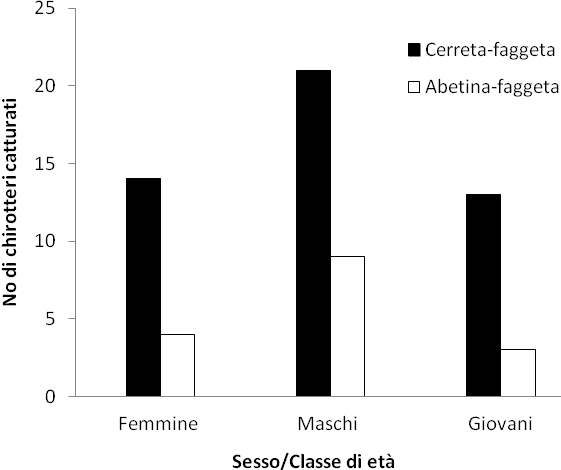
\includegraphics[width=\linewidth]{abstracts/extended_abstracts/P005_Figure1.png}
  \captionof*{figure}{Fig. 1 –  Distribuzione del sesso e delle classi di età (femmine adulte, maschi adulti e giovani) nei chirotteri catturati, per tipologia forestale. Le differenze sono tutte statisticamente significative.}
\end{Figure}


I pipistrelli per ambo sessi e classi di età sono stati catturati in numero significativo nella cerreta-faggeta, rispetto all’abetina-faggeta (femmine adulte: $\chi^2$=5.55, g.d.l.=1, \prob{}-value=0.018; maschi adulti: $\chi^2$=4.80, g.d.l.=1, \prob{}-value=0.028; giovani: $\chi^2$=6.25, g.d.l.=1, \prob{}-value=0.012), (Fig.~1). Le femmine adulte non sono state catturate in numero significativo rispetto ai maschi adulti nella cerreta-faggeta ($\chi^2$=1.40, g.d.l.=1, \prob{}-value=0.237) e nell’abetina-faggeta ($\chi^2$=1.92, g.d.l.=1, \prob{}-value=0.166). Gli adulti, rispetto ai giovani sono stati catturati in numero significativo nella cerreta-faggeta ($\chi^2$=10.08, g.d.l.=1, \prob{}-value=0.001) e nell’abetina-faggeta ($\chi^2$=6.25, g.d.l.=1, \prob{}-value=0.012).

L’indice di cattura calcolato per la cerreta-faggeta è 0.039, mentre per l’abetina-faggeta è 0.013.

\section*{Discussione}
I dati mostrano che il tipo di bosco, la sua struttura e l’altitudine sono in grado di influenzare l’attività dei chirotteri. Inoltre, anche la disponibilità di prede è un fattore che potrebbe favorire l’attività, sebbene nel presente studio non sia stato considerato.

La cerreta-faggeta ha una più elevata ricchezza di specie e dei livelli di attività, a causa sia dell’altitudine, sia dell’eterogeneità strutturale che caratterizza il popolamento. 

Il bosco, specialmente nelle aree più interne è costituito da diversi microhabitat e ha una struttura disetanea, con abbondante necromassa (alberi morti in piedi, rami e alberi caduti a terra) e potenziali \textit{roost} (Fig.~2).    

\begin{Figure}
  \centering\small
  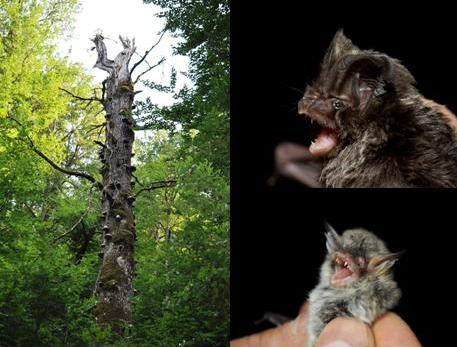
\includegraphics[width=\linewidth]{abstracts/extended_abstracts/P005_Figure2.png}
  \captionof*{figure}{Fig. 2 –  Cerro (\emph{Quercus cerris}) morto in piedi a Bosco Magnano (a sinistra). \emph{Barbastella barbastellus} (in alto, a destra), foto: Antonio Conte. \emph{Myotis nattereri} (in basso, a destra), foto: Serena Di Santo.}
\end{Figure}

Un altro fattore che influenza positivamente l’attività e la disponibilità di insetti è dato dalla presenza del Torrente Peschiera, che attraversa gran parte dell’area forestale. Questa eterogeneità ambientale favorisce la presenza di chirotteri che cacciano sulla volta forestale (es. \emph{N. leisleri}), nello spazio aereo all’interno della foresta e lungo i margini (es. \emph{P. pipistrellus}, \emph{P. pygmaeus}), tra la vegetazione (\emph{P. auritus}, \emph{B. barbastellus}, \emph{M. nattereri}), sulla superficie dell’acqua (\emph{M. daubentonii}). A tal proposito l’uso differenziale dello spazio di foraggiamento, per specie che vivono nella stessa area forestale, può determinare una stratificazione verticale dell’attività in habitat complessi (Francis, 1994; Kalcounis et al., 1999; Hayes et al., 2000). 

L’altitudine e altri fattori geografici possono influenzare anche la distribuzione dei sessi, infatti, le femmine adulte generalmente utilizzano le foreste presenti più a bassa quota, per minimizzare i costi di termoregolazione e incrementare l’efficienza di foraggiamento (Cryan et al., 2000). Le femmine adulte sono state catturate con maggiore frequenza nella cerreta-faggeta, e anche i maschi, sebbene nei mesi estivi tendano a disperdersi fino alle quote elevate, sono stati catturati più frequentemente nella stessa tipologia di bosco. 

Il numero di individui giovani e di femmine adulte catturate tende a eguagliarsi in entrambe le tipologie di bosco e questo fenomeno, per quanto concerne il bosco presente più a bassa quota (cerreta-faggeta), può essere dovuto sia a vantaggi legati alla maggiore disponibilità di prede, sia al mantenimento dei contatti materni (Grindal et al., 1999).

L’indagine svolta rappresenta il primo studio sulla chirotterofauna del Parco Nazionale del Pollino e ha permesso di censire specie rare e di pregio naturalistico e conservazionistico, che rappresentano una componente faunistica importante per gli ecosistemi forestali e sono potenzialmente in grado di influenzare l’organizzazione delle biocenosi (\textit{keystone species}), attraverso il controllo dell’abbondanza di insetti. Importanti sono anche gli habitat oggetto di studio, che pur avendo una limitata estensione, possono contenere risorse chiave (\textit{keystone resources}), come le cavità degli alberi (Cockle et al., 2011) che sono cruciali ai fini della sopravvivenza dei chirotteri e di molte altre specie. 

La ricerca ha permesso anche di indagare la chirotterofauna associata alle faggete degli Appennini con \emph{Abies alba}, che sono un habitat prioritario (cod. 9220$\ast$) per la conservazione, ai sensi della direttiva 92/42/CE. Queste consociazioni sono piuttosto rare in Italia e nella parte meridionale della penisola hanno subito notevoli alterazioni, dovute all’attività antropica fin dall’epoca romana (Susmel, 1959; Ciancio et al., 1985).    

Le informazioni acquisite sono di carattere preliminare, in quanto solo delle indagini pluriannuali possono delineare i \textit{trend} sul grado di frequentazione dell’area di studio, le fluttuazioni dei livelli di attività e le variazioni della ricchezza in specie. A tale proposito assumono particolare importanza le indagini pluriannuali condotte attraverso stime numeriche delle colonie di chirotteri e la valutazione degli indici di attività per valutare gli impatti antropici a breve e a lungo termine, su ecosistemi e biodiversità (Kunz et al., 2009).

I dati circa la fedeltà dei pipistrelli a specifici siti di foraggiamento e di \textit{roosting} all’interno delle aree forestali e l’uso preferenziale di differenti tipologie di boschi, dominati dalla presenza di determinate specie arboree, sebbene siano molto limitati in Italia (Russo et.al. 2004, 2010) possono fornire informazioni utili per la gestione degli habitat e del paesaggio forestale.

Come si evince dal Piano AIB 2012--2014 predisposto dal PN del Pollino, l’Ente si impegna a proporre la promozione e l’attuazione di una gestione forestale sostenibile anche attraverso le attività di formazione per gli operatori del settore. Per questo sarebbe opportuno considerare una gestione forestale orientata alla conservazione, all’incremento dei pipistrelli e dei loro rifugi, sviluppando delle linee guida dettagliate da inserire nei programmi di formazione per le ditte agricolo-forestali e per i tecnici degli Enti locali. 

\vskip3mm

\begin{small}
\noindent\textbf{Ringraziamenti}\\
La ricerca è stata realizzata grazie a un finanziamento dell’Ente Parco Nazionale del Pollino e del MATTM. Le attività di cattura sono state autorizzate dal MATTM su parere dell’ISPRA (prot. PNM-2014-0003894). Si ringrazia sentitamente il Dott. For.le Aldo Schettino (Ente Parco Nazionale del Pollino), l’Isp. Lorenzo Viceconte e l’Agente Gioiadonato (Corpo Forestale dello Stato). 

\vskip3mm

\noindent\textbf{Bibliografia}\\

Anthony E.L.P., 1988. Age determination in bats. In: Kunz T.H. (Ed.) Ecological and Behavioral Methods for the Study of Bats. Smithsonian Institution Press, Washington, DC. 47--58.

Barlow K.E., 1999. Expedition Field Techniques. Bats. The Expedition Advisory Centre, Royal Geographical Society, London.

Blasi C., Burrascano S., Maturani A., Sabatini F.M., 2010. Foreste Vetuste in Italia, Contributo Tematico alla Strategia Nazionale per la Biodiversità. Ministero dell’Ambiente e della Tutela del Territorio e del Mare.

Christensen M., Emborg J., 1996. Biodiversity in natural versus managed forests. Forest Ecology and Management 85: 47--51.

Ciancio O., Iovino F., Menguzzato G., Mirabella A., 1985. L’Abete (\emph{Abies alba} Mill.) in Calabria: possibilità e limiti di diffusione e ridiffusione. Annali Ist. Sper. Selvicoltura, vol. 16: 7--249.

Cockle K.L., Martin K., Wesolowski T., 2011. Woodpeckers, decay, and the future of cavity-nesting vertebrate communities worldwide. Frontiers in Ecology and Conservation 9: 377--382.

Cryan P.M., Bogan M.A., Altenbach J.S., 2000. Effect of elevation on distribution of female bats in the Black Hills, South Dakota. Journal of Mammalogy 81: 719--725.

Dietz C., Von Helversen O., 2004. Illustrated identification key to the bats of Europe. Electronic publication, version 1.0, Tübingen, Germany.

Ente Parco Nazionale del Pollino, 2012. Piano delle Attività di Previsione, Prevenzione e Lotta Attiva contro gli Incendi Boschivi, periodo di validità 2012--2014, redatto dai funzionari: Valicenti A., De Vivo G., Schettino A.

Erkert H.G., 1982. Ecological aspects of bat activity rythms. In: Kunz T.H. (Ed.) Ecology of Bats. Plenum Press, New York. 201--242.

Fenton M.B., 1970. A  technique  for monitoring bat activity with results obtained from different environments in southern Ontario. Canadian Journal of Zoology 48: 847--851;.

Francis C.M., 1994. Vertical stratification of fruit bats (Pteropodidae) in lowland dipterocarp rainforest in Malaysia. Journal of Tropical Ecology 10: 523--530.

Galimberti A., Spada M., Russo D., Mucedda M., Agnelli P., et al., 2012. Integrated Operational Taxonomic Units (IOTUs) in Echolocating bats: a bridge with Molecular  and Traditional Taxonomy. PLoS ONE  7(6): e40122. \url{doi:10.1371/journal.pone.0040122}
  
Grindal S.D., Morrissette J.l., Brigham R.M., 1999. Concentration of bat activity in riparian habitats over an elevational gradient. Canadian Journal of Zoology 77: 972--977.

Harmon M.E., Franklin J.F., Swanson F.J., Sollins P., Gregory S.V., Lattin J.D., Anderson N.H., Cline S.P., Aumen N.G., Sedell J.R., Lienkaemper G.W., Cromack K. Jr., Cummins K.W., 1986. Ecology of coarse woody debris in temperate ecosystems. Advances in Ecological  Researchs 15: 133

Hayes J.P., Gruver J.C., 2000. Vertical stratification of bat activity in an old-growth forest in western Washington. Northwest Science 74: 102--108.

Kalcounis M.C., Hobson K.A., Brigham R.M., Hecker K.R., 1999. Bat activity in the boreal forest: importance of stand type and vertical strata. Journal of Mammalogy 80: 673--682.

Kunz T.H., Brock C.E., 1975. A comparison of mist nets and ultrasonic detectors for monitoring flight activity of bats. Journal of Mammalogy 58: 309--315.

Kunz T.H., Parsons S., 2009. Ecological and Behavioral Methods for the Study of Bats, 2\textsuperscript{nd} Editiln. The Johns Hopkins University Press.

Nòrden B., Appelqvist T., 2001. Conceptual problems of ecological continuity and its bioindicators. Biodiversity and Conservation 10: 779--791.

O'Donnell C.F.J., 2000. Influence of season, habitat, temperature and invertebrate availability of nocturnal activity of the New Zealand long-tailed bat (\emph{Chalinolobus tuberculatus}). N.Z.J. Zool. 27: 207--221.

Russo D., Jones G., 2000. The two cryptic species of \emph{Pipistrellus pipistrellus} (Chiroptera: Vespertilionidae) occur in Italy: evidence from echolocation and social calls. Mammalia 64: 187--197;.

Russo D., Cistrone L., Jones G., et al., 2004. Roost selection by Barbastelle bats (\emph{Barbastella barbastellus}, Chiroptera: Vespertilionidae) in beech woodlands of central Italy: consequences for conservation. Biol. Conserv. 117: 73--81.

Russo D., Cistrone L., Garonna A.P., Jones G., 2010. Reconsidering the importance of harvested forests for the conservation of tree-dwelling bats. Biodivers. Conserv. 19: 2501--2515.

Whitloch M.C., Schluter D., 2010. Analisi statistica dei dati biologici. Zanichelli.

Worthington-Wilmer J., Barratt E.M., 1996. A nonlethal method of tissue sampling for genetic studies of chiropterans. Bat Research News 37: 1-–3.

\end{small}

\end{multicols}
% % EOF % %